\documentclass[11pt, oneside]{memoir}   	% use "amsart" instead of "article" for AMSLaTeX format
\usepackage{geometry}                		
\usepackage{blindtext}
\usepackage[utf8]{inputenc}
\usepackage{amsmath}
\usepackage[greek,english]{babel}
\usepackage{alphabeta}
\geometry{letterpaper}                   		% ... or a4paper or a5paper or ... 
%\geometry{landscape}                		% Activate for rotated page geometry
%\usepackage[parfill]{parskip}    		% Activate to begin paragraphs with an empty line rather than an indent
\usepackage{graphicx}				% Use pdf, png, jpg, or eps§ with pdflatex; use eps in DVI mode
% TeX will automatically convert eps --> pdf in pdflatex		
\usepackage{amssymb}
\usepackage{xcolor}
\usepackage{tcolorbox}
\usepackage{pgfplots}
\usepackage{braket}
\usepackage{tikz}
\usepackage{circuitikz}
\usepackage{float}
\usetikzlibrary{patterns,positioning}


%------FOR DARK MODE USE-------
%\pagecolor[rgb]{0.2,0.2,0.2}
%\color[rgb]{1,1,1}
%------------------------------

%SetFonts

%SetFonts

\newcommand{\definition}[1]{
	\begin{tcolorbox}[colback=blue!5!white,colframe=blue!75!black,title=\textbf{Ορισμός}]
		\begin{center}
			#1
		\end{center}
	\end{tcolorbox}
}

\newcommand{\property}[1]{
	\begin{tcolorbox}[colback=red!5!white,colframe=red!75!black,title=\textbf{Ιδιότητα}]
		\begin{center}
			#1
		\end{center}
	\end{tcolorbox}
}

\newcommand{\suggestion}[1]{
	\begin{tcolorbox}[colback=green!5!white,colframe=green!75!black,title=\textbf{Πρόταση}]
		\begin{center}
			#1
		\end{center}
	\end{tcolorbox}
}

\newcommand{\note}[1]{
	\begin{tcolorbox}[colback=yellow!5!white,colframe=yellow!75!black,title=\textbf{Σημείωση}]
		\begin{center}
			#1
		\end{center}
	\end{tcolorbox}
}


\title{Διεργασίες Κατασκευής Μίκρο και Νάνο Συστημάτων}
\author{Κωνσταντίνος Ζουριδάκης}
\date{}							% Activate to display a given date or no date

\begin{document}
\maketitle
\section{Διάλεξη 02/10/2024}

\subsection{Διαδικαστικά}

\textbf{Προτείνεται διάβασμα διαφανειών μετά από κάθε διάλεξη (τουλάχιστον μία ώρα την εβδομάδα) και λύση ασκήσεων του βιβλίου}.

Αποτελείται από:
\begin{itemize}
	\item 2 εργασίες (30\%)
		\begin{itemize}
			\item  1 εργασία με θέμα υπολογιστικό λιθογραφίας.
			\item 1 εργασία με θέμα την ενχάραξη.
		\end{itemize}
		
	\item 1 γραπτή εξέταση (70\%)
\end{itemize}

Τα βιβλία είναι:

\begin{itemize}
	\item \textbf{Silicon VLSI Technology}
	\item Introduction to Microfabrication
\end{itemize}

Θα γίνει και χρήση κάποιων λογισμικών για χάραξη με πλάσμα.

\subsection{Μάθημα}

\begin{center}
	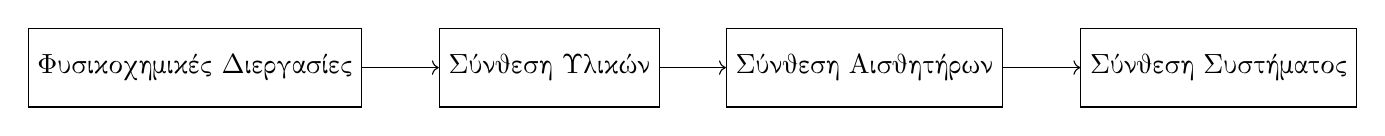
\begin{tikzpicture}
		% Draw the first block
		\node (block1) [draw, rectangle, minimum width=2cm, minimum height=1cm] {Φυσικοχημικές Διεργασίες};
		
		% Draw the second block next to the first one
		\node (block2) [draw, rectangle, minimum width=2cm, minimum height=1cm, right of=block1, node distance=4.5cm] {Σύνθεση Υλικών};
		
		% Draw the third block next to the second one
		\node (block3) [draw, rectangle, minimum width=2cm, minimum height=1cm, right of=block2, node distance=4cm] {Σύνθεση Αισθητήρων};
		
		% Draw the fourth block next to the third one
		\node (block4) [draw, rectangle, minimum width=2cm, minimum height=1cm, right of=block3, node distance=4.5cm] {Σύνθεση Συστήματος};
		
		% Connect the blocks with arrows
		\draw[->] (block1) -- (block2);
		\draw[->] (block2) -- (block3);
		\draw[->] (block3) -- (block4);
	\end{tikzpicture}
\end{center}

\subsection{MOSFET Transistor}

\note{MOSFET $\rightarrow$ Metal-Oxide Semiconductor Field Effect Transistor }

Η διάταξη ενός MOSFET παρουσιάζεται παρακάτω.

\begin{center}
	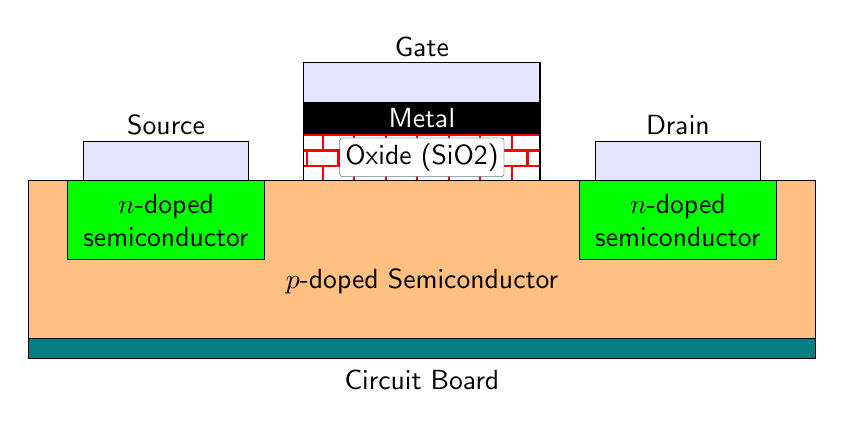
\begin{tikzpicture}[font=\sffamily]
		\draw[fill = teal] (0,0) rectangle (10,-0.25) node[below=1ex, midway] {Circuit Board};
		\draw[fill=orange!50] (0,0) rectangle (10,2) node [below,midway] {$p$-doped Semiconductor};
		
		% Oxide part (lower part)
		\draw[pattern=bricks, pattern color=red] (3.5,2) rectangle (6.5,2.6) node[midway, fill=white, inner sep=2pt, draw, ultra thin, rounded corners=1] {Oxide (SiO2)};
		
		% Metal part (upper part)
		\draw[fill=black] (3.5,2.6) rectangle (6.5,3) node[midway, text=white, inner sep=2pt, draw, ultra thin, rounded corners=1] {Metal};
		
		
		\draw[fill=blue!10] (3.5,3) rectangle (6.5,3.5) node[above=6pt, midway] {Gate};
		\draw[fill=blue!10] (0.5+0.2,2) rectangle (3-0.2,2.5) node[above=6pt, midway] {Source};
		\draw[fill=blue!10] (10-0.5-0.2,2) rectangle (10-3+0.2,2.5) node[above=6pt, midway] {Drain};
		
		\draw[fill=green] (0.5,1) rectangle (3,2) node[midway, align=center] {$n$-doped\\semiconductor};
		
		\draw[fill=green] (10 - 0.5,1) rectangle (10 - 3,2) node[midway, align=center] {$n$-doped\\semiconductor};
		
	\end{tikzpicture}
\end{center}

\subsection{pn junction}

Ένα p-n junction είναι ένας συνδυασμός από δύο τύπου ημιαγωγικά υλικά, p-type και n-type. Στο \textcolor{blue}{n} κομμάτι κινούνται \textcolor{blue}{ελεύθερα ηλεκτρόνια}, ενώ στο \textcolor{red}{p} κομμάτι κινούνται \textcolor{red}{ελεύθερες ωπές} (σημεία που λείπουν ηλεκτρόνια). Όταν αυτά τα δύο κομμάτια ενωθούν, δημιουργείται το \textbf{depletion region} στο οποίο τα ελεύθερερα ηλεκτρόνια γεμίζουν τις ωπές, αυτό με τη σειρά του επιτρέπει το ρεύμα να κινείται μόνο προς μία κατεύθυνση.


Όταν συνδεθεί σε κύκλωμα λειτουργεί σαν δίοδος η οποία αποσκοπεί ακριβώς στο να μεταφέρει το ρεύμα μόνο προς μία κατεύθυνση.




\begin{center}
	
	\begin{figure}[H]
		\centering
		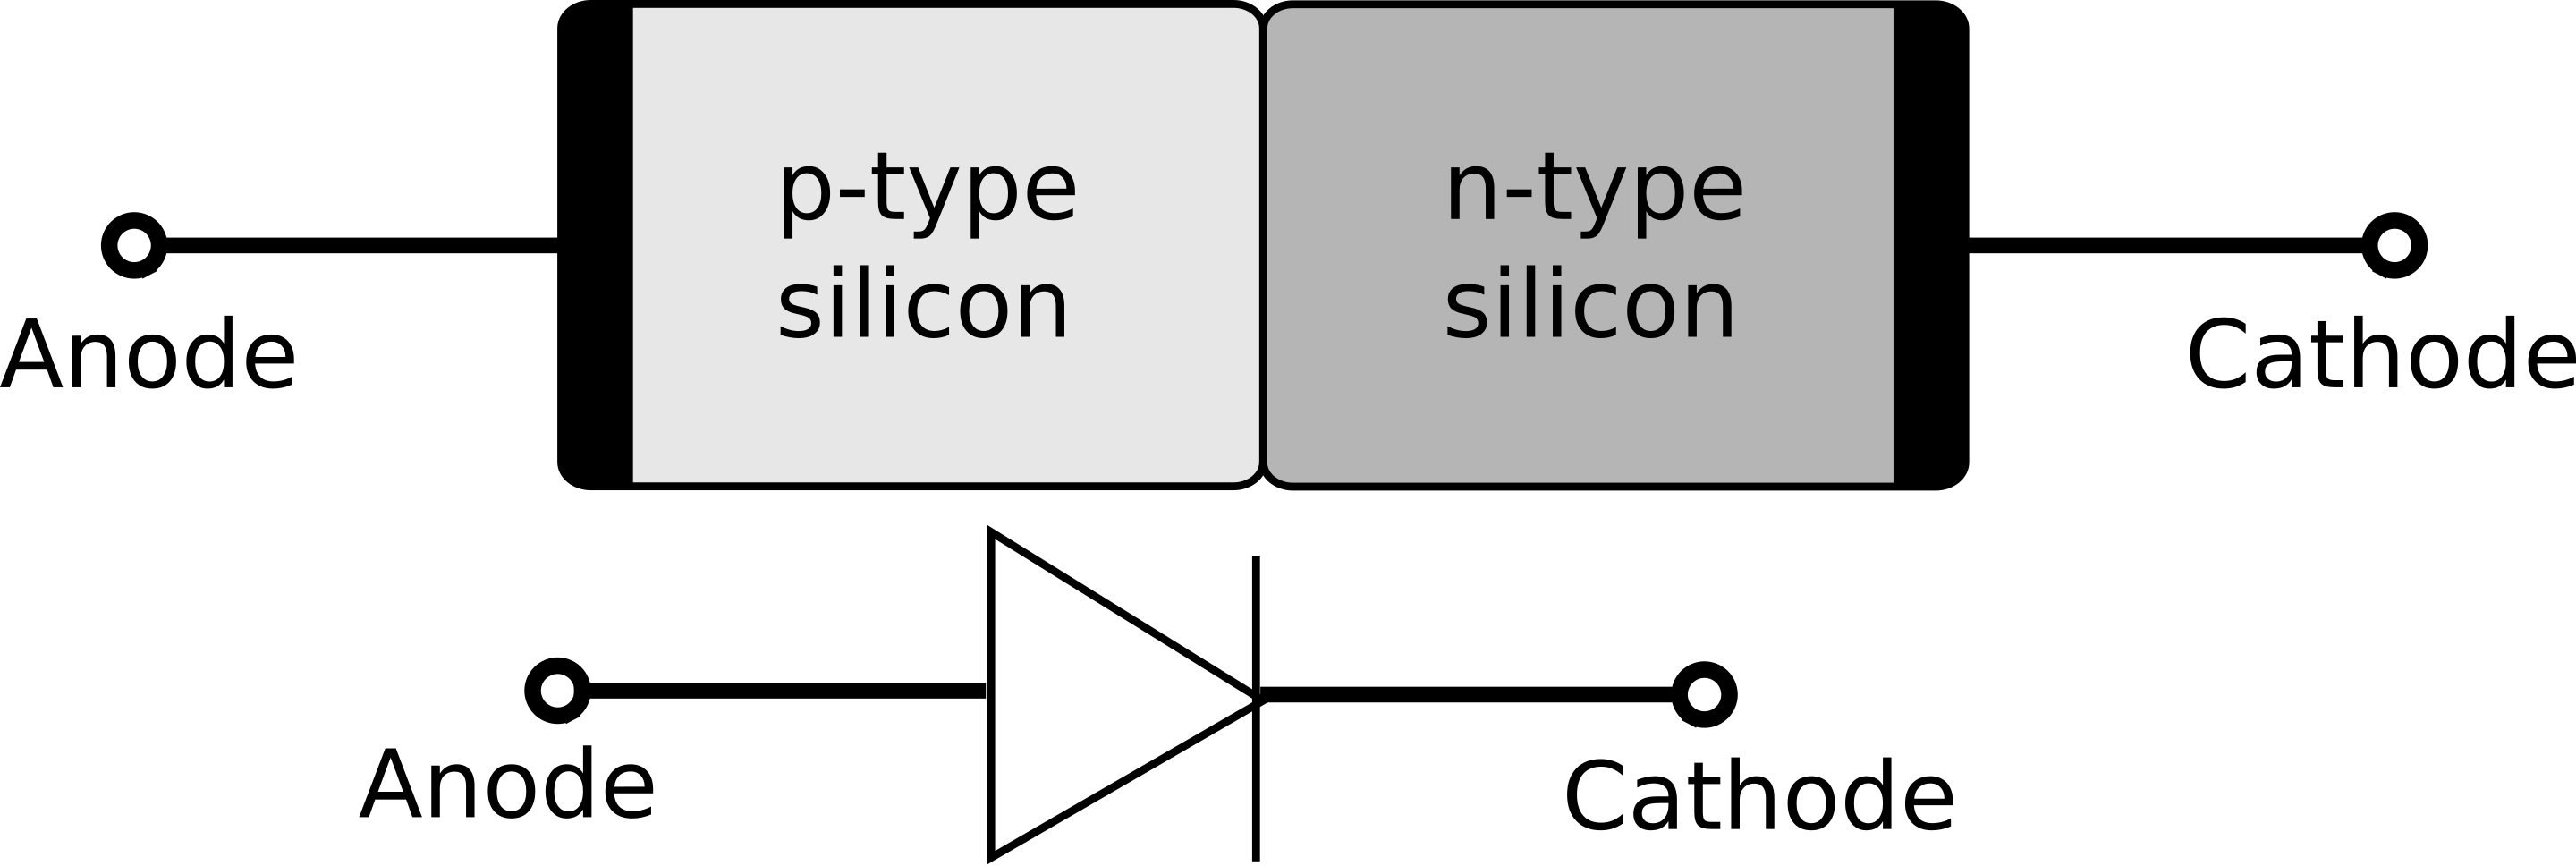
\includegraphics[width=0.7\linewidth]{Pictures/diode}
		\caption{pn junction. Από κάτω εμφανίζεται το σύμβολο της διόδου.}
		\label{fig:diode}
	\end{figure}
	
	\begin{figure}[H]
		\centering
		\includegraphics[width=0.7\linewidth]{"Pictures/Screenshot 2024-10-06 at 12.57.31 PM"}
		\caption{Forward bias. Στην περίπτωση αυτή δημιουργείται ηλεκτρικό πεδίο αντίστροφο από αυτό που δημιουργείται από την επαφή και μόνο των p και n υλικών με αποτέλεσμα να μικραίνει το depletion region. Depletion region υπάρχει αν εφαρμόσουμε τάση από 0 - 0.6 Volt, από 0.6 Volt και πάνω θεωρητικά δεν υπάρχει αντίσταση οπότε το ρεύμα ρέει ανεμπόδιστα.}
		\label{fig:screenshot-2024-10-06-at-12}
	\end{figure}
	
	\begin{figure}[H]
		\centering
		\includegraphics[width=0.7\linewidth]{"Pictures/Screenshot 2024-10-06 at 12.58.49 PM"}
		\caption{Reverse bias. Στην περίπτωση αυτή δεν ρέει ρεύμα.}
		\label{fig:screenshot-2024-10-06-at-12}
	\end{figure}
\end{center}


\subsection{npn transistor}
\begin{figure}[H]
	\centering
	\includegraphics[width=0.7\linewidth]{"Pictures/Screenshot 2024-10-06 at 1.07.04 PM"}
	\caption{Ένα npn transistor. Αποτελείται από δύο διόδους συνδεδεμένες back-to-back. Η μία δίοδος είναι η Emitter-Base δίοδος και η άλλη είναι η Collector-Base δίοδος.}
	\label{fig:screenshot-2024-10-06-at-1}
\end{figure}

\begin{figure}[H]
	\centering
	\includegraphics[width=0.7\linewidth]{"Pictures/Screenshot 2024-10-06 at 1.08.08 PM"}
	\caption{Τα states στα οποία μπορεί να βρίσκεται το npn transistor (BJT). Στο cutoff mode λειτουργεί σαν ανοιχτό κύκλωμα, δηλαδή δεν περνάει ρεύμα. Στο saturation mode λειτουργεί σαν κλειστό κύκλωμα, δηλαδή σαν "καλώδιο". Το πιο σημαντικό είναι το \textbf{active mode}. Στο active mode αυξάνεται η ένταση του ρεύματος.}
	\label{fig:screenshot-2024-10-06-at-1}
\end{figure}

\begin{figure}[H]
	\centering
	\includegraphics[width=0.7\linewidth]{"Pictures/Screenshot 2024-10-06 at 1.10.41 PM"}
	\caption{npn transistor σε active mode.}
	\label{fig:screenshot-2024-10-06-at-1}
\end{figure}

\subsection{Διαδικασία Λιθογραφίας}

\begin{figure}[H]
	\centering
	\includegraphics[width=0.7\linewidth]{"Pictures/Screenshot 2024-10-06 at 1.12.42 PM"}
	\caption{Διαδικασία Λιθογραφίας.}
	\label{fig:screenshot-2024-10-06-at-1}
\end{figure}

\subsection{Επίπεδο Fermi}

Το επίπεδο Fermi ουσιαστικά είναι το υψηλότερο ενεργειακό επίπεδο στο οποίο μπορεί να μεταβεί ένα ηλεκτρόνιο.

\subsection{Διάφορες Πληροφορίες}

3 ηλεκτρονιοβόλτ $\rightarrow$ Ημιαγωγος\\
Αν $>$ 3 ηλεκτρονιοβόλτ $\rightarrow$ Μονωτής

Πυρίτιο ντοπαρισμένο με φώσφορο = n-τυπου $\rightarrow$ Αρνητική αγωγιμότητα \\
Πυρίτιο ντοπαρισμένο με βόριο = p-τυπου $\rightarrow$ Θετική αγωγιμότητα.

Εφαρμόζοντας διαφορετικές τάσεις κάθε φορά μπορούμε να κάνουμε τον αγωγό τύπου n, intristic, τύπου p.

\end{document}  